\documentclass[11pt]{article}

\usepackage[margin=1.5in]{geometry}

\usepackage{fancyhdr}
\pagestyle{fancy}
\newcommand\course{ASTR 101}
\newcommand\hwnumber{3}
\newcommand\duedate{October 14, 2020}

\lhead{Oliver Tonnesen\\V00885732}
\chead{\textbf{\Large Lab \hwnumber{} Report}}
\rhead{\course\\\duedate}

\usepackage[
	backend=biber,
	url=true
]{biblatex}
\addbibresource{lab3.bib}
\usepackage{enumitem}
\usepackage{graphicx}
\usepackage{url}
\usepackage{pgfplots}
\pgfplotsset{width=10cm,compat=1.9}

\usepackage{multirow}

\usepackage{amsmath,amsfonts}
\DeclareMathOperator{\km}{km}
\DeclareMathOperator{\px}{px}


\begin{document}
\section{Objective}
This labe exercise studies the Sun's rotation by comparing a series of images taken of one of its sunspots over the course of seven days.


\section{Introduction}
Even before observing its rotation directly, we have several other reasons to believe that the Sun might rotate.
First of all, every other object in the universe seems to rotate in some way; whether it's a planet, another star, or a galaxy, cosmic objects always seem to be spinning.
A slightly more direct indicator that the Sun should be spinning is that it was formed from a cloud of spinning gas.
The rotational energy contained in this gas cloud should not simply disappear because the gas took on a new form, so we expect that the Sun should conserve this rotational energy.


\section{Procedure}
Using GIMP, the eight images were superimposed onto one another to obtain the image seen in Figure~\ref{img:sunspots}.
The central point of each sunspot was estimated by a point, a line of best fit was drawn through each of these points.
Using the line of best fit as a baseline, we drew a semicircle to estimate where the sunspots lay on the surface of the Sun.
Finally, the angles from the centre of the Sun projected onto this semicircle to each of the points was measured.
These projections can be found with and without Figure~\ref{img:sunspots} underlying it in Figure~\ref{img:sunspots_projections} and Figure~\ref{img:projections}, respectively.
From these measurements, we calculated the period of rotation of the Sun.


\section{Calculations}
\subsection{Sunspot Width} \label{sec:sunspot_width}
The width of the Sun in our images was measured to be 1 870 pixels.
The diameter of the Sun is known to be approximately 1 392 500 km.
We measured the sunspot to be either 28 pixels or 57 pixels, depending on whether the orange ring around the cool centre is considered to be a part of the sunspot.

The ratio between the actual width of the sunspot and the actual width of the Sun should be the same as the width between the width of the sunspot and the width of the Sun as measured in the images, so we can estimate the actual width of the sunspot as follows:
\begin{equation}
\label{eqn:sunspot_width_centre}
\begin{split}
	\textrm{Width of sunspot (centre only)}
	&= 1\;392\;500\;\km \cdot \frac{28\;\px}{1\;870\;\px}\\
	&\approx 20\;850\;\km
\end{split}
\end{equation}
and
\begin{equation}
\label{eqn:sunspot_width_ring}
\begin{split}
	\textrm{Width of sunspot (orange ring included)}
	&= 1\;392\;500\;\km \cdot \frac{57\;\px}{1\;870\;\px}\\
	&\approx 42\;445\;\km
\end{split}
\end{equation}


\subsection{Solar Period}
To estimate the solar period at each measurement, we simply divide 360 by the difference in angle between the observed position of the sunspot after one day.
A sample calculation cna be seen below, using the difference in angle between the observation on April 10 and April 11:
\begin{equation}
\begin{split}
	\textrm{Period} &= \frac{360^\circ}{57.84^\circ - 43.82^\circ} * 1\;\textrm{day}\\
			&\approx 25.68\;\textrm{days}
\end{split}
\end{equation}

To find the uncertainty, we calculate the sample standard deviation of the set of calculated solar periods using the following formula:
\begin{align*}
	s = \sqrt{\frac{1}{N-1}\sum^N_{i=1} \left(x_i-\overline{x}\right)^2}
\end{align*}
Where $N$ is the number of samples, $\overline{x}$ is our sample mean, and each $x_i$ is a solar period computed between two consecutive days.
Plugging in the values from Table~\ref{table:sunspot_displacements}, we get $s \approx 0.85$.


\subsection{Sidereal Solar Period} \label{sec:sidereal_period}
Adding $1^\circ$ to each of the values in the third column of Table~\ref{table:sunspot_displacements}, we get the following new values:
\newline
\newline
\begin{tabular}{| c |}
	\hline
	15.02\\ \hline
	14.94\\ \hline
	14.62\\ \hline
	15.02\\ \hline
	13.86\\ \hline
	15.04\\ \hline
	14.64\\ \hline
\end{tabular}
\newline
\newline
The mean of these values is about 14.73.
Repeating the calculation of the solar period using this new value, we get the following solar period:
\begin{equation}
\begin{split}
	\textrm{Solar period} &= \frac{360}{14.73}\\
			      &\approx 24.43
\end{split}
\end{equation}


\section{Answers}
\begin{enumerate}[label={\textbf{\emph{(\arabic*)}}}]
	\item % 1
To most accurately calculate the width of the sunspot, we chose the image taken on April 13, when the sunspot was most directly facing the camera.
Measuring only the coolest part of the sunspot in its centre, the width is 28 pixels.
Measuring the entire spot including the orange, the width is 37 pixels.
This gives us diameters of approximately 20 850 km and 42 445 km, respectively.
The calculations resulting in these estimates can be seen in Section~\ref{sec:sunspot_width} in Equations~\ref{eqn:sunspot_width_centre} and~\ref{eqn:sunspot_width_ring}.

	\item % 2
If sunspots are fixed, then they should move the same amount when viewed at the same time each day; in our observations, their positions vary in difference by up to $1^\circ$.
The changes in angle measured from our images can be found in column 3 of Table~\ref{table:sunspot_displacements}.

	\item % 3
		The sunspots may have shifted to a different latitude throughout the course of our observations, possibly causing (in part) the discrepancies we noticed in \textbf{\emph{(2)}}.

	\item % 4
The Greeks believed that the Earth was at the centre of the universe, and that the Sun orbited around it~\cite{lecture-slides}.
The observation of sunspots proved that this was not the case, and in fact it is the Earth that orbits the Sun.

	\item % 5
Using the values in the ``change in angle'' column of Table~\ref{table:sunspot_displacements}, we calculate the solar period to be approximately 26.21days, over 1.5 days longer than we expect it to be at the solar equator.
The Earth moves about $1^\circ$ in its orbit each day.
This means that in each observation after the first, our view of the Sun has moved $1^\circ$.
We can correct for this by simply adding $1^\circ$ to each entry in the ``change in angle'' column of Table~\ref{table:sunspot_displacements}.
Re-calculating the solar period with these new values (seen in Section~\ref{sec:sidereal_period}), we get a sidereal period of 24.43 days, which is much closer to the solar period we expect at the equator.
\end{enumerate}


\section{Discussion}
This lab exercise demonstrated how to estimate the solar rotational period from a sample of images a sunspot over the course of several days.
We saw how to project these images of the sunspot onto a semicircle representing the surface of the Sun, and use this projection to measure the difference in the angle at which we viewed the sunspot on consecutive days.

When measuring this angle, we corrected for the Earth's rotation about the Sun by adding $1^\circ$ to each measured difference in angle.
Some other possible sources of error in our estimations are the fact that the sunspot might have drifted slightly to a different location on the surface of the Sun in between observations, causing our projections to be inaccurate, and also human error in making the various measurements of our projections.


\section{Conclusion}
In this lab exercise, we learned about the Sun's rotation and how to calculate it from daily images of one of its sunspots, along with some factors we had to consider to improve the accuracy of these calculations.
We also saw how these observations were made and used by Galileo in the early 1600s to prove that the Earth orbited the Sun.


\section{Observations, Tables, and Graphs}
\begin{table}[h]
\caption{Angular displacements of a sunspot.}
\renewcommand{\arraystretch}{1.5}
\begin{tabular}{| c | c | c | c |}
	\hline
	Date & Angle (deg) & Change in angle (deg) & Solar Period (days)\\ \hline
	April 10 & 43.82 & -- & --\\ \hline
	April 11 & 57.84 & 14.02 & 25.68\\ \hline
	April 12 & 71.78 & 13.94 & 25.82\\ \hline
	April 13 & 85.40 & 13.62 & 26.43\\ \hline
	April 14 & 99.42 & 14.02 & 25.68\\ \hline
	April 15 & 112.28 & 12.86 & 27.99\\ \hline
	April 16 & 126.32 & 14.04 & 25.64\\ \hline
	April 17 & 139.96 & 13.64 & 26.39\\ \hline
	\multicolumn{3}{| c |}{\textbf{Average Period \& Uncertainty}} & $26.23 \pm 0.85$\\
	\hline
\end{tabular}
\label{table:sunspot_displacements}
\end{table}

\begin{figure}[h]
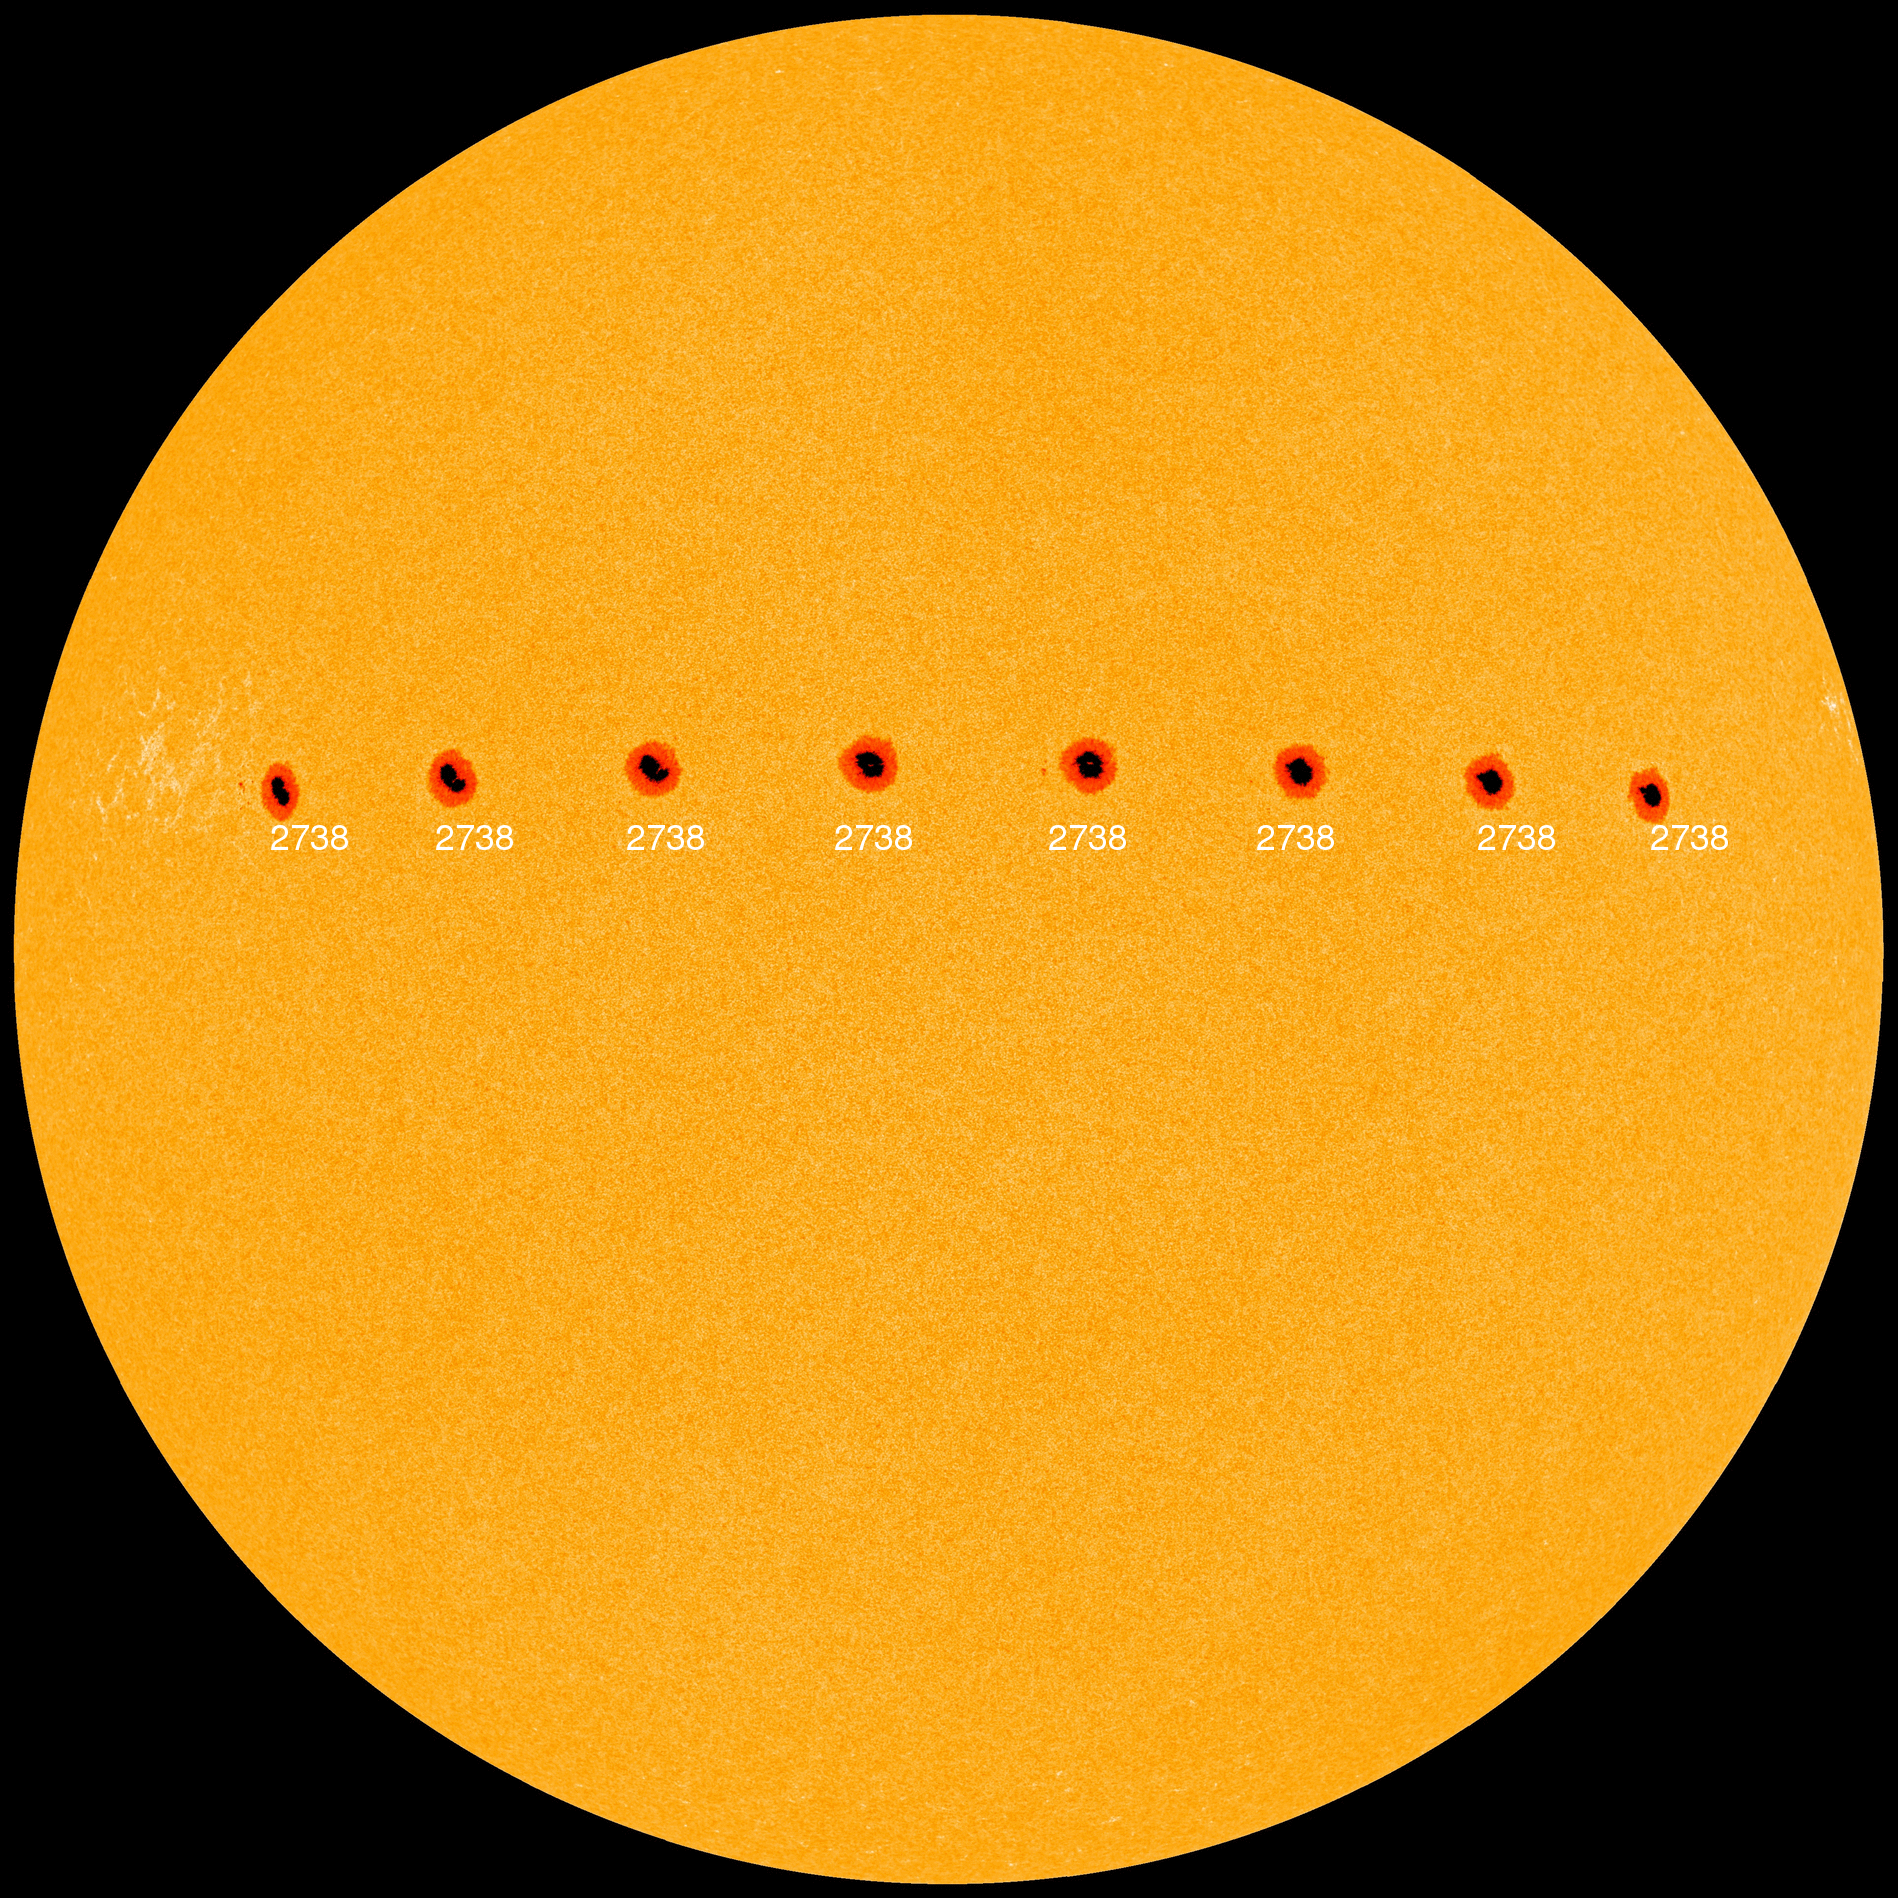
\includegraphics[width=\columnwidth]{figures/sunspots.png}
\caption{The eight sunspot images superimposed on one another.}
\label{img:sunspots}
\end{figure}

\begin{figure}[h]
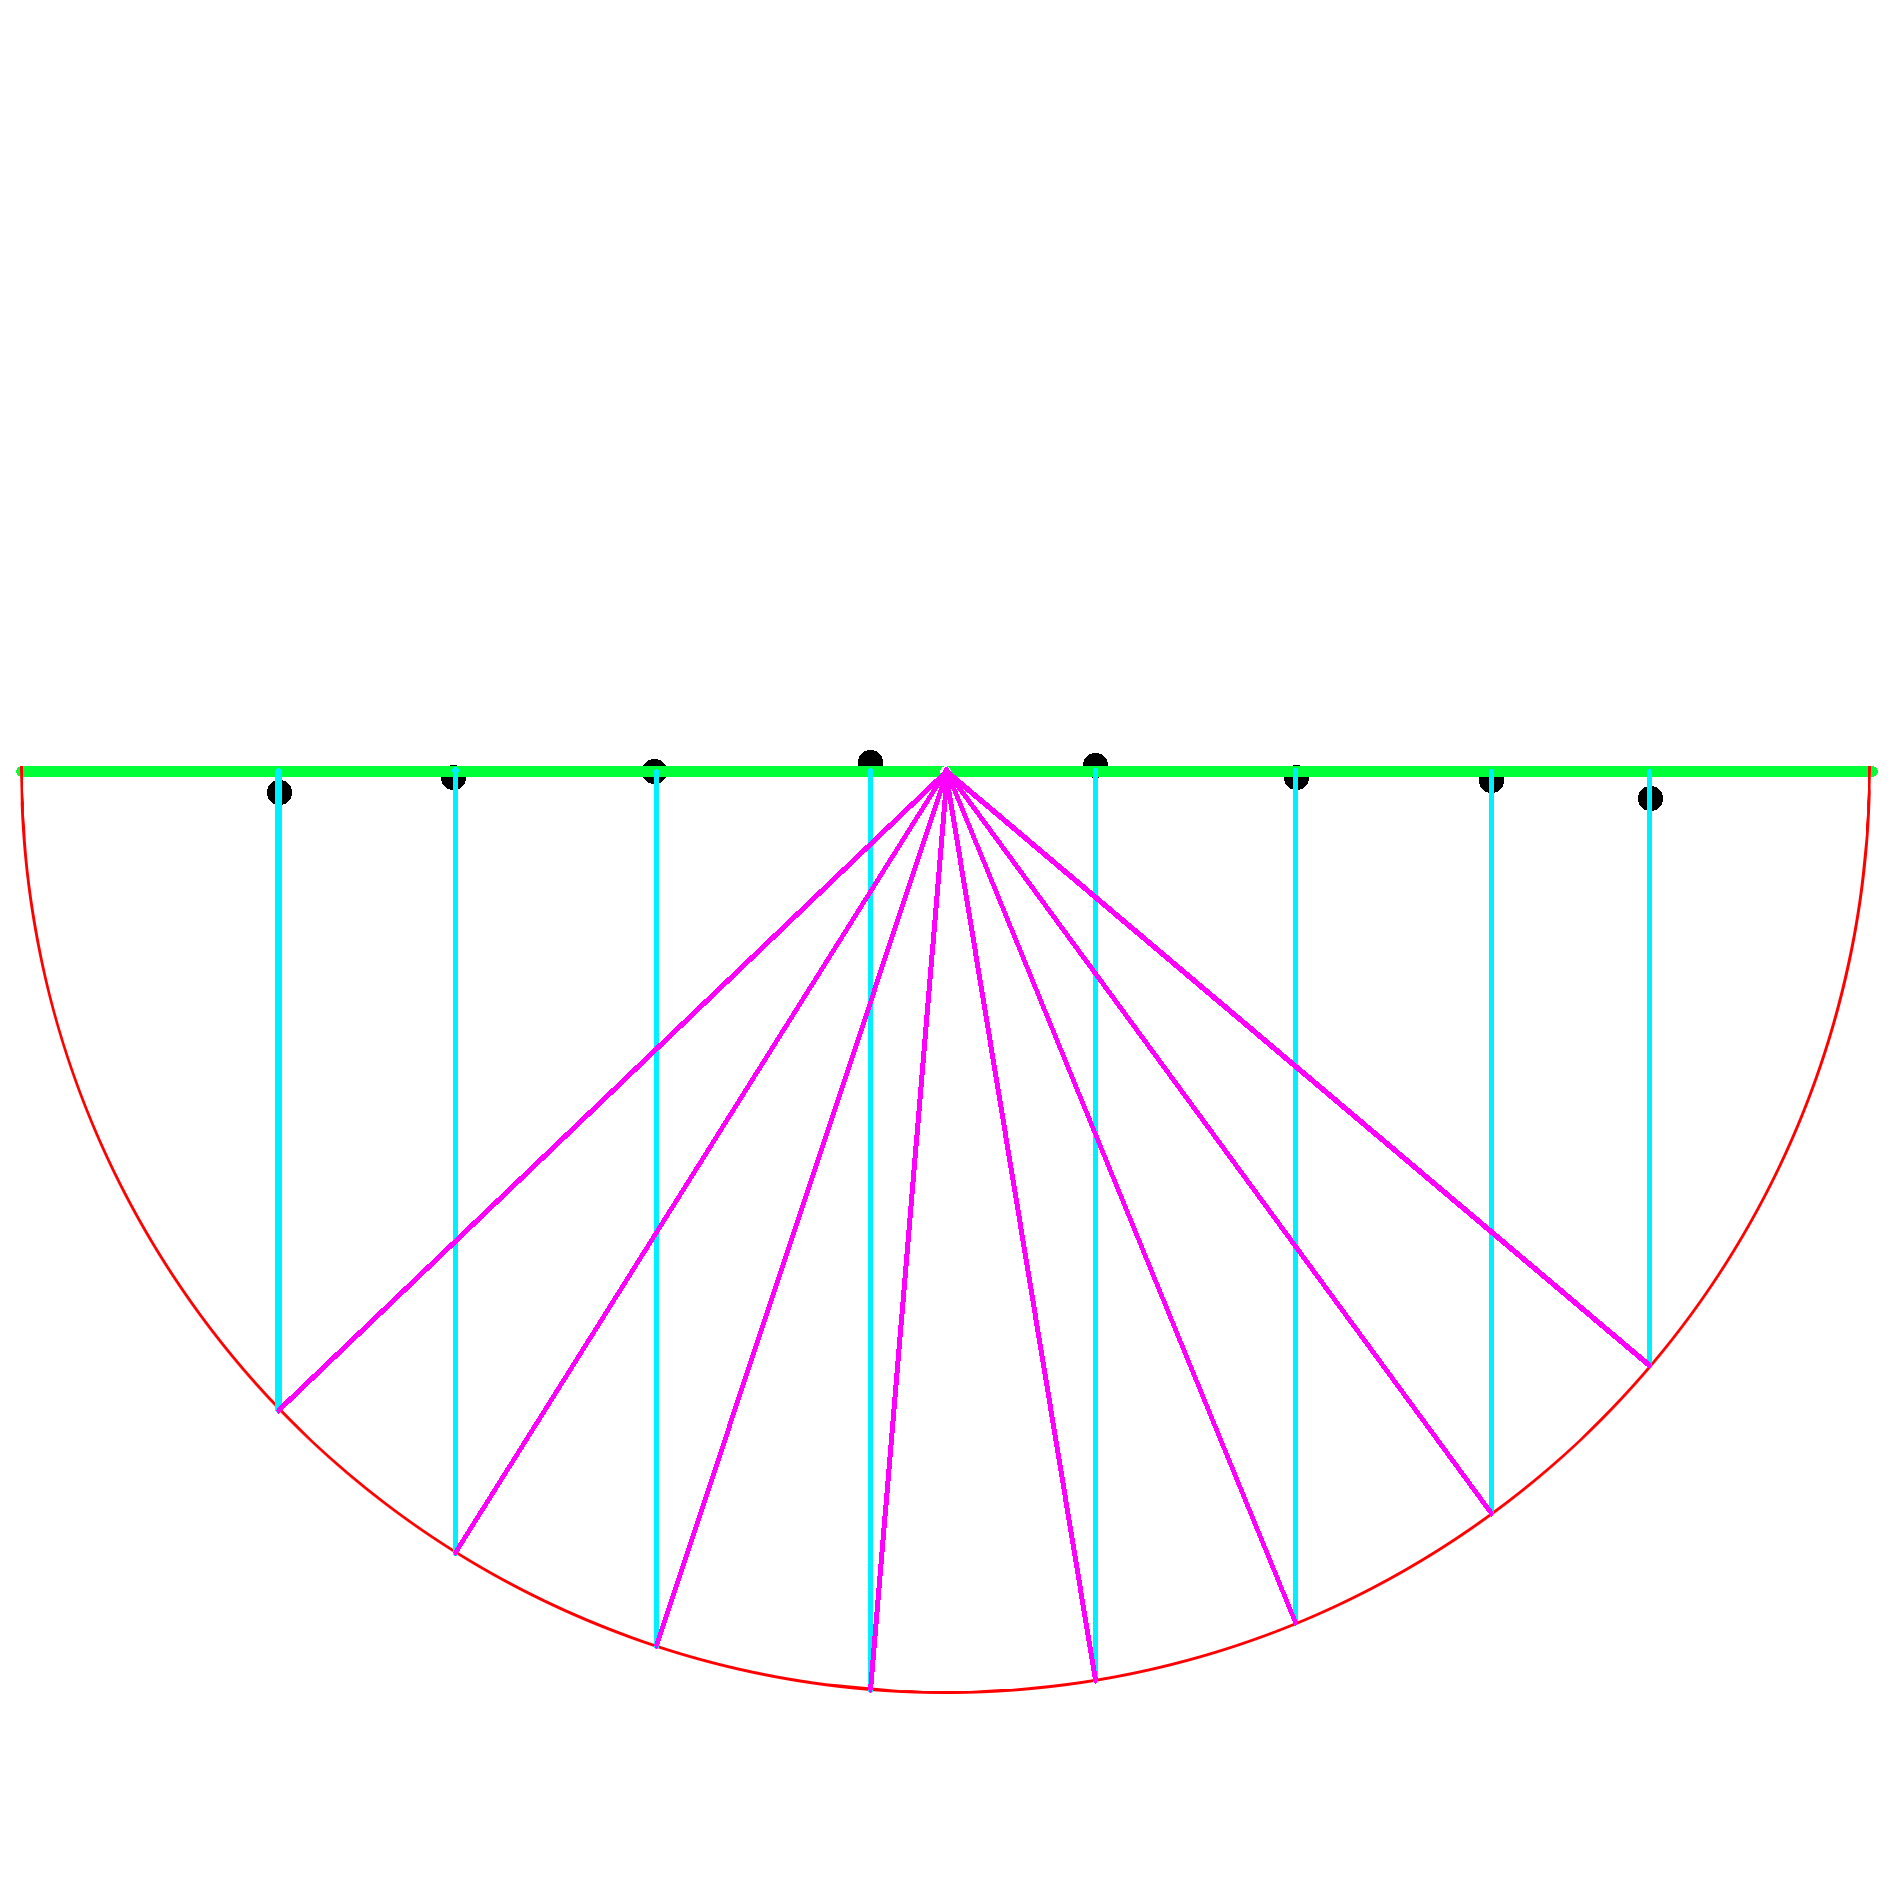
\includegraphics[width=\columnwidth]{figures/projections.png}
\caption{Projections of the sunspots onto the surface of the Sun.}
\label{img:projections}
\end{figure}

\begin{figure}[h]
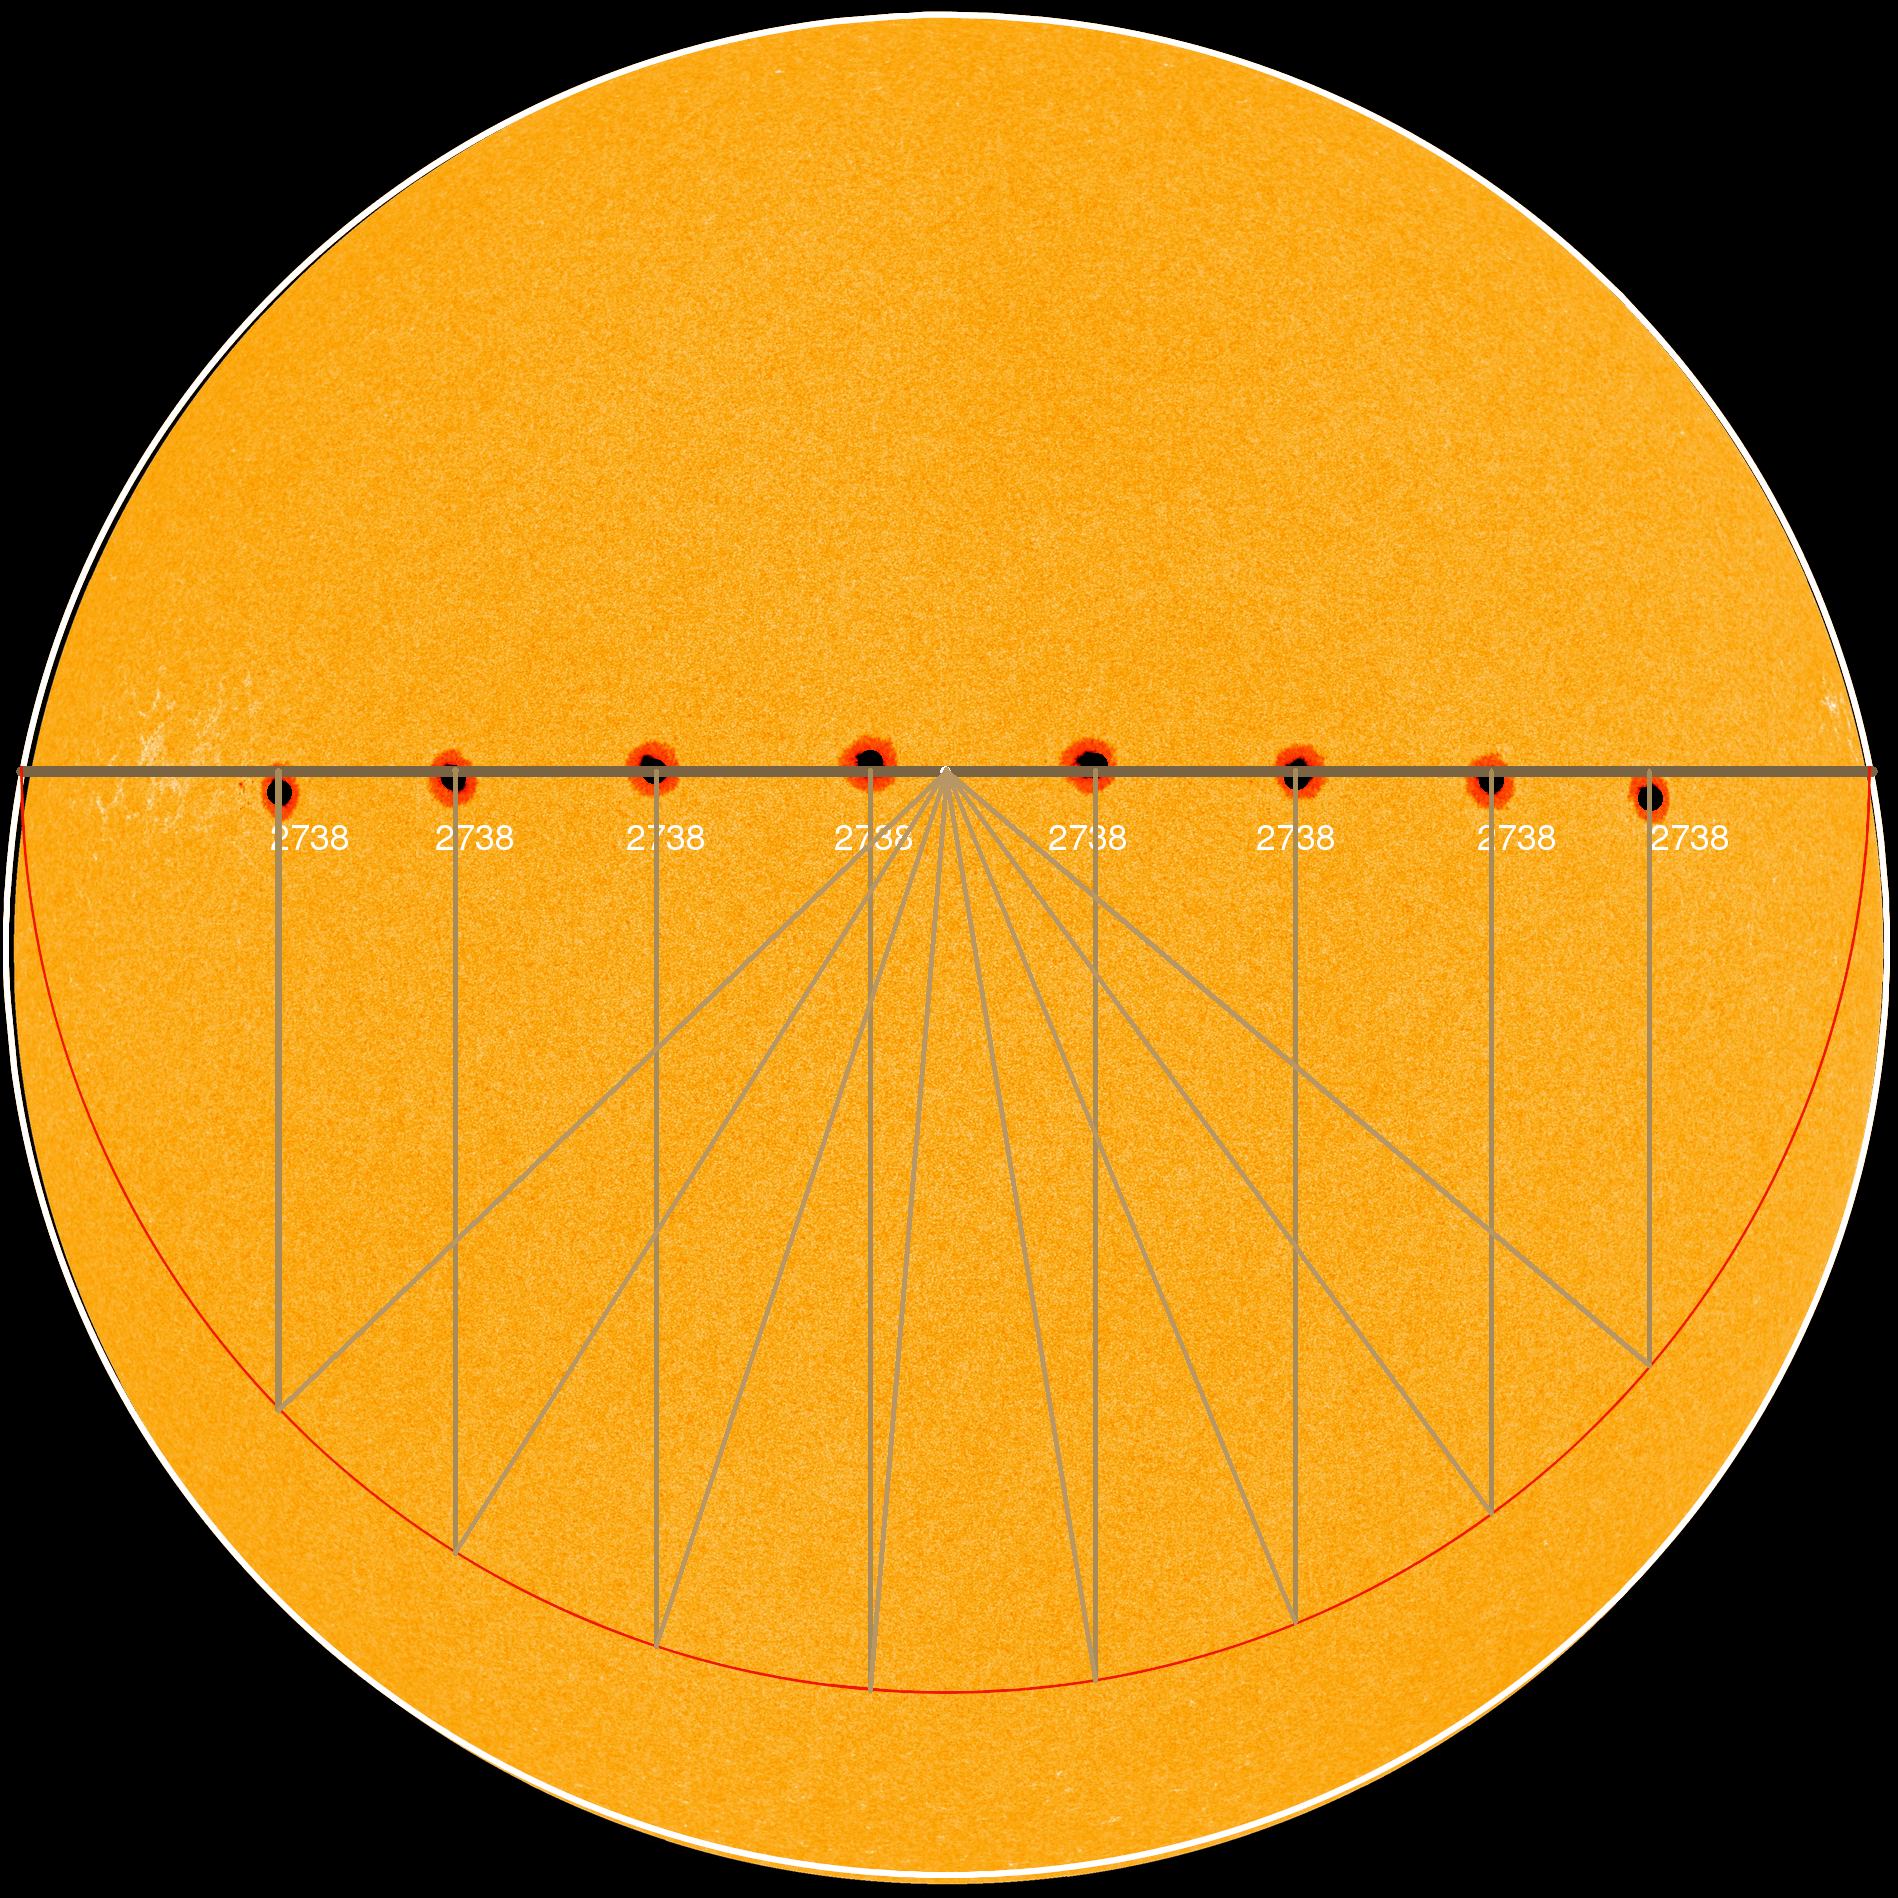
\includegraphics[width=\columnwidth]{figures/sunspots_projections.png}
\caption{Figure~\ref{img:sunspots} overlain by the projections of the sunspots onto the surface of the Sun in Figure~\ref{img:projections}.}
\label{img:sunspots_projections}
\end{figure}

\begin{figure}[h]
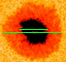
\includegraphics[width=\columnwidth]{figures/sunspot_width.png}
\caption{Width of the sunspot, using either only the darkest part in the centre (top line), or the entire spot including the orange (bottom line).}
\label{img:sunspot_width}
\end{figure}


\printbibliography


\end{document}
